\section{Objectives and approach\label{section:inductive-objectives-and-approach}}

This section provides a characterization of the synthesis problem and an overview of our solution. Section~\ref{subsection:inductive-synthesis-statement} makes this problem more precise in terms of the models from Chapter~\ref{chapter:framework}. Section~\ref{subsection:inductive-synthesis-requirements} states additional requirements on the synthesis approach; the problem statement can be strengthened to take each of them into account. Section~\ref{subsection:inductive-synthesis-approach} presents an overview of our inductive approach in the light of these requirements.

%%%

\subsection{Problem statement\label{subsection:inductive-synthesis-statement}}

In its simplest form, the problem of synthesizing LTS state machines from MSC scenarios can be stated as follows:

\begin{quote}
\underline{Given}~a consistent MSC collection showing typical examples and counterexamples of system behaviors:
\begin{align*}
Sc = (S^+,S^-),
\end{align*}
\underline{Synthesize}~the system as a composition of agent LTSs:
\begin{align*}
System = (Ag_1 \parallel \ldots \parallel Ag_n)
\end{align*}
\underline{Such that}~$Sc$ and $System$ are consistent.
\end{quote}

The consistency condition covers the three following criteria, discussed in Section~\ref{subsection:background-scenario-consistency}.

\begin{description}
\item[Structural consistency:] the state machine and scenario views are \emph{structurally} consistent, that is, they agree on the agent decomposition and their respective interface.

\item[Consistent agent view:] each timeline of the positive scenarios in $S^+$ specifies an existing path in the corresponding agent state machine. Similarly, each timeline of the positive precondition of a negative scenario in $S^-$ specifies an existing path in the corresponding agent state machine. 

\item[Consistent system view:] the system covers all positive scenarios and the preconditions of all negatives ones; it also excludes all negative scenarios. The precise conditions from Section~\ref{subsection:background-scenario-consistency} are:
\begin{align}
&\mathcal{L}^+(Sc) \subseteq \mathcal{L}(System)         \label{relation:inductive-statement-positive}\\
&\mathcal{L}^-(Sc) \cap \mathcal{L}(System) = \emptyset, \label{relation:inductive-statement-negative}
\end{align}
where $\mathcal{L}^+(Sc)$ and $\mathcal{L}^-(Sc)$ encode the scenario collection in terms of positive and negative event traces, respectively.

\end{description}

%%%

\subsection{Requirements on the synthesis approach\label{subsection:inductive-synthesis-requirements}}

The above characterization provides a precise and minimal statement in terms of the formal models of Chapter~\ref{chapter:framework}. It may be further completed with the following requirements.

\begin{description}
\item[Behavior generalization] -- Scenarios provide only \emph{examples} of system behaviors; they are thus incomplete. The synthesized state machines should cover more behaviors than those provided as input. 

Covering more behaviors is allowed by our formal statement but not enforced. The \emph{consistent system view} condition states an upper bound on behavior generalization by requiring negative scenarios to be excluded. This upper bound needs to be refined if other models are to be taken into account (see below).

\item[Incremental synthesis] -- Rather than requiring the whole scenario collection to be available at the beginning, the synthesis should accommodate new scenario examples and counterexamples incrementally as they arise during the synthesis process.
\begin{itemize}

\item End-users are most likely unable to provide a comprehensive set of scenarios from the beginning, including state assertions along scenario episodes or flowcharts on such episodes. The synthesis approach should therefore work even if only a few scenarios are available when the synthesis starts.

\item Both positive and negative scenarios should be taken into account. Negative scenarios appear fairly common in the material provided by stakeholders. They naturally illustrate violations of implicit goals in a way easier to specify.

\item In an interactive approach, a more comprehensible set of scenarios is likely to be \emph{eventually} available. The synthesis should smoothly accommodate new scenarios and further information arising in the later phases of the synthesis. For example, the synthesis should be able to take a hMSC as input. 

\end{itemize}

\item[Multi-view synthesis] -- The possibility of ``richer'' input specifications should be taken into account in the synthesis process, such as fluents or goals. Such specifications are not \emph{required} as input; they may however improve the synthesis when available. 

\noindent Our problem statement must therefore be strengthened: 
\begin{itemize}
\item All models used as input at some stage or another of the synthesis are required to be consistent with each other. 
\item The synthesized output system itself must be consistent with all such models. In particular, the synthesized system may not violate safety goals if the latter are provided as input.
\end{itemize}

\end{description}

The incremental integration of those requirements in our approach will drive the structure of this chapter. The next section provides an overview of the synthesis process.

%%%

\subsection{Overview of our inductive approach to synthesis\label{subsection:inductive-synthesis-approach}}

Figure~\ref{image:inductive-synthesis-overview} shows the two main steps of our approach for the simple case where a scenario collection is taken as input. 

\begin{figure}[h]
\centering
\scalebox{0.63}{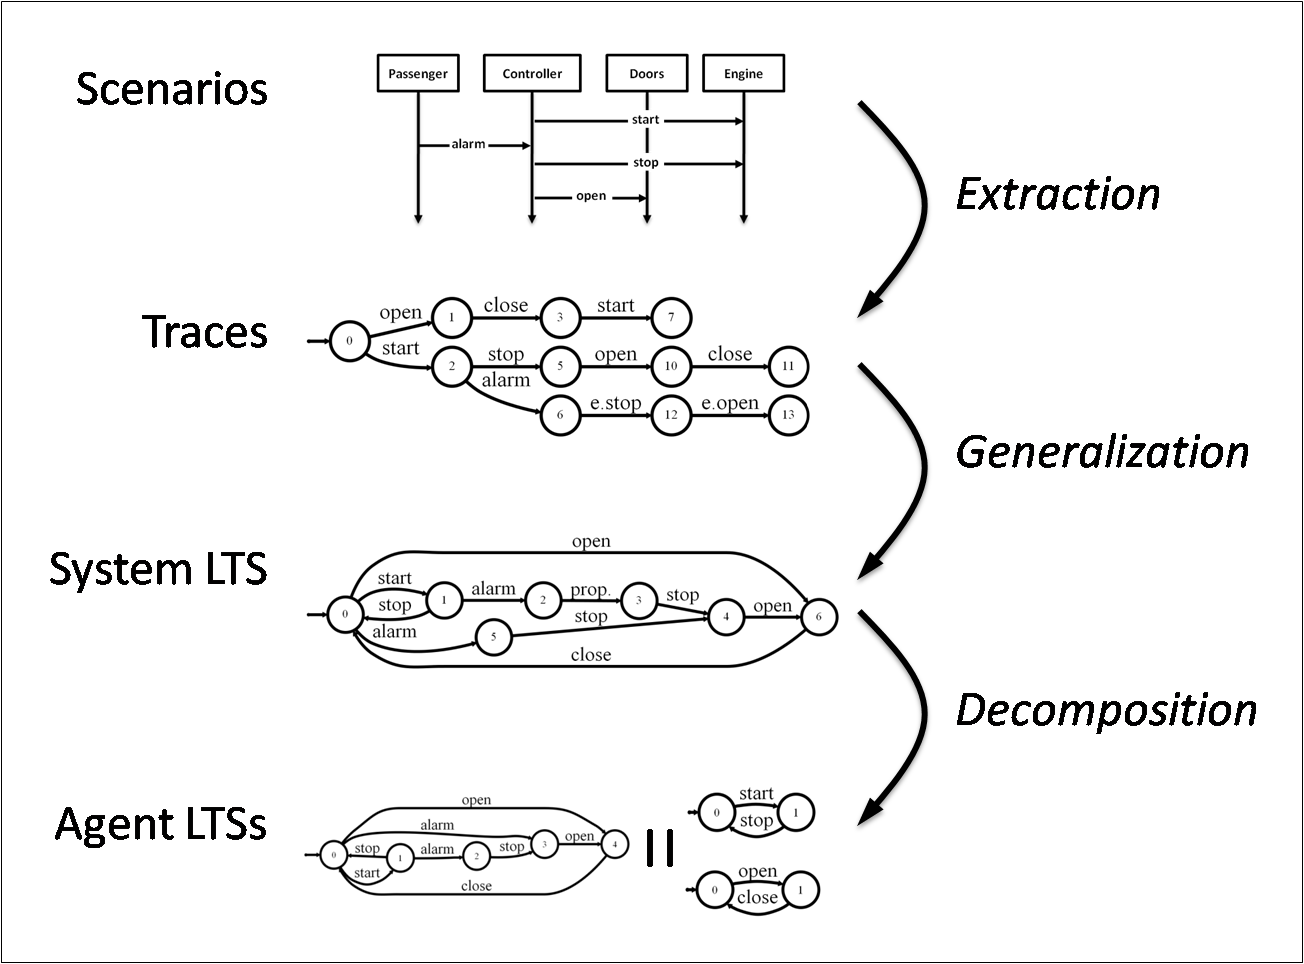
\includegraphics[trim=3mm 3mm 3mm 3mm, clip]{src/4-inductive/images/overview}}
\caption{Inductive LTS synthesis from MSCs: overview\label{image:inductive-synthesis-overview}}
\end{figure}

\subsubsection*{The generalization step}

This step extends grammar induction techniques developed in \cite{Oncina:1992} to synthesize a system LTS covering all positive traces and excluding all negative ones. The generalization strategy is borrowed from the RPNI algorithm (RPNI stands for Regular Positive and Negative Inference) developed in the context of grammar induction \cite{Oncina:1992}, see Section \ref{section:inductive-background} hereafter. Roughly, it proceeds as follows.

An initial LTS $A_0$ is built as a first solution; it has the shape of a tree that accepts all positive scenario traces but does not generalize behaviors. To achieve such generalization, the initial LTS is incrementally refined as automata $A_1,\ldots,A_n$ by merging well-chosen state pairs (see Fig.~\ref{Fig:algo:steps} on page~\pageref{Fig:algo:steps} for an illustration of this process).

This process is such that the two relations below hold. Relation~(\ref{equation:generalization-step-1}) states that the initial LTS $A_0$ is a valid solution when it comes to accepting the positive traces. Relation~(\ref{relation:inductive-language-refinements}) states that the generalization process is monotonic in that the behaviors accepted by an intermediate solution will remain accepted by every of its successors, up to the final LTS $A_n$.
\begin{align}
&\mathcal{L}^+(Sc) = \mathcal{L}(A_0) \label{equation:generalization-step-1}\\
&\mathcal{L}(A_0) \subseteq \mathcal{L}(A_1) \subseteq \ldots \subseteq \mathcal{L}(A_n)
\label{relation:inductive-language-refinements}
\end{align}

To avoid overgeneralization, this process is performed under the control of the negative traces from $\mathcal{L}^-(Sc)$. Every intermediate solution $A_i$ has to meet the \emph{consistent system view} condition; the latter provides a useful algorithm invariant, namely,
\begin{align}
&\mathcal{L}^+(Sc) \subseteq \mathcal{L}(A_i)        \label{relation:inductive-invariant}\\
&\mathcal{L}^-(Sc) \cap \mathcal{L}(A_i) = \emptyset \label{relation:inductive-invariant-II}
\end{align}

This invariant provides a proof argument if compared to relations (\ref{relation:inductive-statement-positive}) and (\ref{relation:inductive-statement-negative}). Correctness arguments will be detailed in Section~\ref{XXX}.

\subsubsection*{The decomposition step}

In a second step, a LTS for each agent is computed by projecting the system LTS onto their respective alphabet. For an agent $Ag$ the projection of the system LTS $S$ is given by:
\begin{align}
(S \setminus \Sigma_{Ag}^c)^\Delta
\end{align}
\noindent where $\Sigma_{Ag}^c$ denotes the set of all system events excluding those of $Ag$'s interface.

The above formula makes use of the hiding, determinization and minimization operators on LTS discussed in Section~\ref{section:background-state-machines}.

\subsubsection*{Meeting additional requirements}

As we just mentioned it, the generalization step is driven by RPNI; Section \ref{section:inductive-background} provides some background on this grammar induction approach. However, this is just a first milestone toward an inductive LTS synthesis approach that meets all requirements in Section \ref{subsection:inductive-synthesis-requirements}. 
\begin{itemize}
\item Scenario behaviors are generalized without requiring additional state or flowchart information. 
\item RPNI does not support incremental system synthesis; multi-model consistency is not guaranteed either. 
\end{itemize}

Section~\ref{section:lts-induction-from-mscs} will therefore introduce the Query-driven State Merging (QSM) algorithm that extends RPNI with features for user interaction and incremental generalization. QSM supports the elicitation of additional, ``interesting'' scenarios that were not originally supplied by the end-user. The original collection of scenarios is completed by asking the user scenario queries that are generated during synthesis. A \emph{scenario query} consists of showing the user a specific scenario, asking her to classify it as positive or negative. Answers to such queries guide the generalization process towards more accurate state machines while incrementally enriching the initial scenario collection.

Our multi-view synthesis requirement is tackled in Section~\ref{section:inductive-mutliview-consistency}. QSM is extended there so as to allow the injection of additional information that constrains the induction and prunes the inductive search space for better performance. Such additional information may include global definitions of fluents; declarative domain properties; behavior models of external components; and goals that the system is expected to satisfy. The extended QSM thereby guarantees the consistency of synthesized state machines with all other models.

Managing the consistency of a large scenario collection is challenging; hMSCs partly address this through a structured form of scenarios (see Section \ref{subsection:background-hmsc}). Section~\ref{section:inductive-from-hMSC} shows how hMSCs can be added to scenario collections as input of the generalization process. In this setting, negative scenarios and other models can still be used to constrain induction so as to achieve multi-view consistency. Accepting hMSCs as input also allows us to remove some assumptions about input scenarios the were required by the previous algorithms.

Taking hMSCs as input implies both a theoretical and practical shift of perspective. It leads us considering the generalization of state machines under the control of safety goals as a synthesis technique that naturally succeeds the generalization of positive scenario behaviors under the control of negative ones. Among others, this perspective is further discussed in Section~\ref{section:inductive-discussion}.
